\section{习题 2.6：二次曲面（8 题）}\label{sec:26}
\tip{\textbf{识别二次曲面的总顺序：}先看二次项正负号（决定椭球、双曲面、抛物面），再看一次项与常数项（决定中心 / 顶点、是否有实点），最后用 $x=h,y=h,z=h$ 的平面截线核查类型。}
\begin{center}
\begin{tikzpicture}[scale=.85,>=Stealth]
\draw[->] (0,0)--(4,0) node[right]{$x$};
\draw[->] (0,0)--(0,3.3) node[above]{$z$};
\draw[blue,thick] plot[smooth] coordinates {(.3,.15)(.5,.45)(.8,1)(1.3,1.9)(1.8,3.05)};
\draw[blue,thick] plot[smooth] coordinates {(-.3,.15)(-.5,.45)(-.8,1)(-1.3,1.9)(-1.8,3.05)};
\draw[dashed,teal] (-1.2,1.75)--(1.2,1.75);
\node at (6.7,2.45) {$z=A x^2+B y^2$};
\node at (6.7,1.8) {截面 $z=h$ 是椭圆};
\node at (6.7,1.15) {若系数异号则是双曲抛物面};
\end{tikzpicture}
\end{center}

\begin{center}
\begin{minipage}{.47\linewidth}\centering
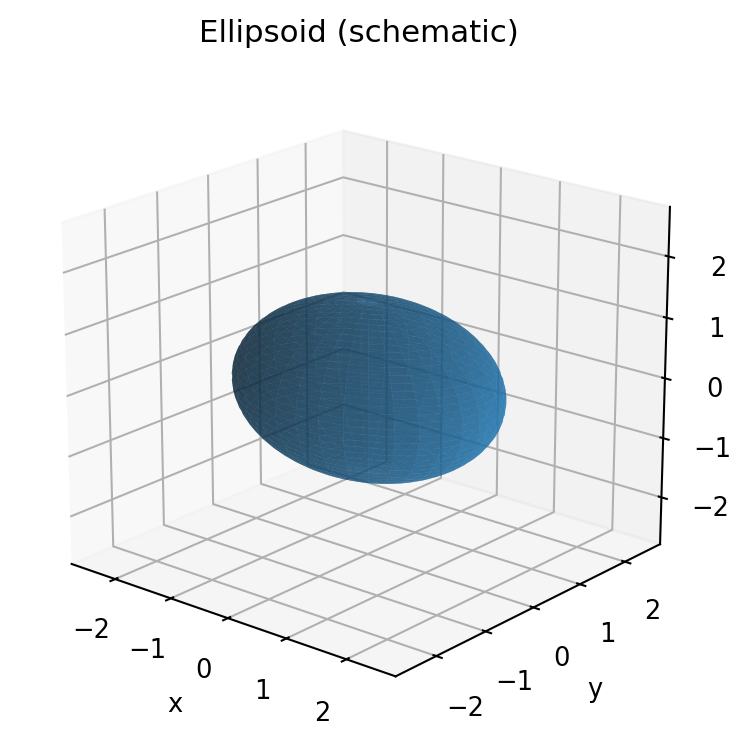
\includegraphics[width=\linewidth]{figures/ellipsoid.png}
{\small\color{navy}椭球面：三个方向上的半轴不一定相等}
\end{minipage}\hfill
\begin{minipage}{.47\linewidth}\centering
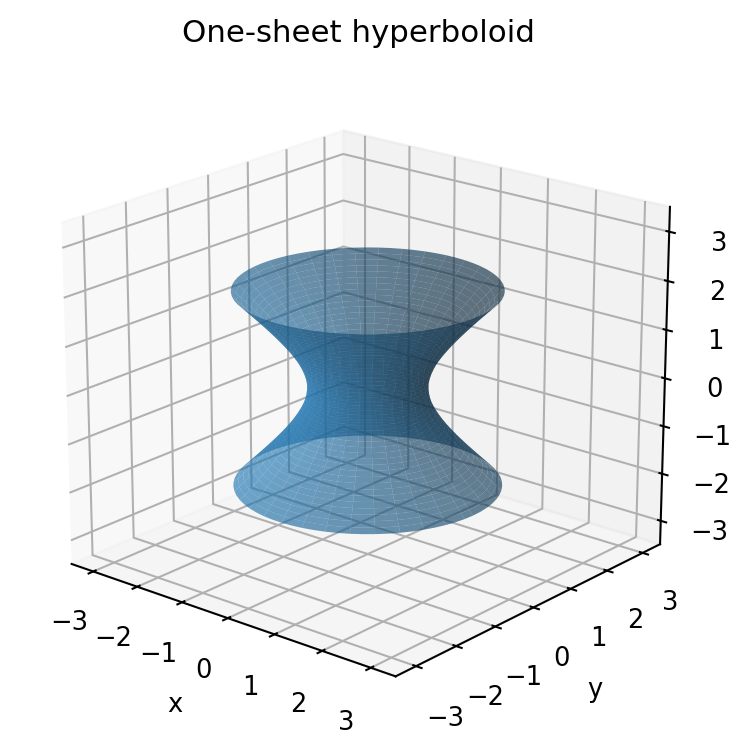
\includegraphics[width=\linewidth]{figures/one-sheet-hyperboloid.png}
{\small\color{navy}单叶双曲面：沿一条轴截面随高度变化}
\end{minipage}
\end{center}
\Q{1}{由两个坐标平面反射对称推出轴对称}
若曲面 $S$ 关于 $xy$ 平面和 $xz$ 平面都对称，则反射变换
\[(x,y,z)\mapsto(x,y,-z),\qquad (x,y,z)\mapsto(x,-y,z)\]
都保持 $S$ 不变。先后施行二者的复合变换
\[(x,y,z)\mapsto(x,-y,-z)\]
恰是绕 $x$ 轴旋转 $180^\circ$，亦即关于 $x$ 轴的轴对称。
\ans{得证；关键是“两个互相垂直平面反射的复合是绕其交线半周旋转”。}

\Q{2}{由三坐标面对称与截圆确定椭球面}
曲面关于三个坐标平面都对称，且为椭球面，所以标准式为
\[\frac{x^2}{a^2}+\frac{y^2}{b^2}+\frac{z^2}{c^2}=1.\]
在 $z=0$ 的截圆 $x^2/9+y^2/16=1$ 说明 $a^2=9,b^2=16$。又点 $(1,2,\sqrt{23})$ 在曲面上，代入有
\[\frac19+\frac4{16}+\frac{23}{c^2}=1 \Rightarrow c^2=36.\]
\ans{$\displaystyle \frac{x^2}{9}+\frac{y^2}{16}+\frac{z^2}{36}=1$，与原书一致。}

\Q{3}{三类二次曲面的方程}
\begin{enumerate}[label=(\arabic*)]
\item 椭圆抛物面：顶点 $O$，关于 $xz,yz$ 对称，故设 $z=Ax^2+By^2$。代入点 $(1,2,5)$ 与 $(\tfrac13,-1,1)$，解
\[A+4B=5,\quad A/9+B=1\Longrightarrow A=9/5,\ B=4/5.\]
\ans{$\displaystyle\frac{x^2}{4}+\frac{y^2}{9}=\frac{5z}{36}$，亦即 $9x^2+4y^2=5z$。}
\item 马鞍面：关于 $xz$ 与 $yz$ 平面都对称，并过 $(1,2,0),(2,0,2),O$。设 $z=Ax^2-By^2$，代入得 $4A=2$、$A-4B=0$，解出 $A=1/2,B=1/8$。\ans{$x^2-y^2/4=2z$。}
\item 关于 $xy,yz$ 平面均对称，曲面上有 $x^2=6y,z=0$ 与 $z^2+4y=0,x=0$ 两条抛物线。设 $y=Ax^2+Bz^2$，代入分别有 $A=1/6,B=-1/4$，所以
\ans{$2x^2-3z^2-12y=0$。}
\end{enumerate}

\Q{4}{根据两条水平截线反推二次曲面}
曲面关于三个坐标平面对称，设为 $Ax^2+By^2+Cz^2=1$（或与其等价的非零倍数）。两条水平截线都给出关于 $A,B,C$ 的比例约束；代入每条截线的 $z$ 值、比较椭圆长短轴即得。结果为：
\begin{enumerate}[label=(\arabic*)]
\item 截线在 $z=\sqrt3$ 时为 $x^2/16+y^2/36=1$，在 $z=2\sqrt2$ 时为 $x^2/36+y^2/81=1$，得到
\[\boxed{\frac{x^2}{4}+\frac{y^2}{9}-z^2=1}.\]
核查：代 $z=\sqrt3$ 得 $x^2/4+y^2/9=4$，两边除 $4$ 恰为题给第一条截线。
\item 截线在 $z=\sqrt3$ 时为 $x^2+y^2/4=1$，在 $z=-\sqrt2$ 时为 $x^2/2+y^2/8=1$，得到
\[\boxed{\frac{x^2}{4}+\frac{y^2}{16}+\frac{z^2}{4}=1}.\]
\item 截线在 $z=4$ 时为 $x^2/9+y^2/18=1$，在 $z=-6$ 时为 $x^2/24+y^2/48=1$，得到
\[\boxed{\frac{x^2}{3}+\frac{y^2}{6}-\frac{z^2}{4}=-1}.\]
\end{enumerate}
\ans{三个式子与原书书后答案一致；建议逐一把两个指定 $z$ 值代回去复验。}

\Q{5}{证明双曲面以圆锥为渐近锥面}
给定
\[F(X)=\frac{x^2}{a^2}+\frac{y^2}{b^2}-\frac{z^2}{c^2}=\pm1\]
及齐次锥面 $F(Y)=0$。设 $X=R\omega$（$|\omega|=1$），则 $F(\omega)=\pm R^{-2}\to0$，说明远离原点时，双曲面点的方向越来越接近锥面在单位球上的交线。
因为在该交线上 $\nabla F\ne0$，由局部可微与紧性可知，可沿单位球小幅转动 $O(R^{-2})$ 找到 $F(\omega_*)=0$。令 $Y=R\omega_*$，就有
\[|X-Y|=R|\omega-\omega_*|=O(R^{-1})\xrightarrow{R\to\infty}0.\]
\ans{从双曲面到锥面的最短距离趋于 $0$；这给出原书“渐近锥面”的严谨量化解释。}

\Q{6}{三轴椭球的两张圆截面}
给定 $a>b>c>0$，椭球
\[\frac{x^2}{a^2}+\frac{y^2}{b^2}+\frac{z^2}{c^2}=1.\]
由于中间半轴为 $b$，若用一张经过 $y$ 轴的平面截取椭球，使它在该平面内的另一正交方向上的二次型系数也恰为 $1/b^2$，则截线为圆。
令平面另一单位方向为 $v=(\cos\theta,0,\sin\theta)$，要求
\[\frac{\cos^2\theta}{a^2}+\frac{\sin^2\theta}{c^2}=\frac1{b^2}.\]
解得
\[\cos^2\theta=\frac{a^2(b^2-c^2)}{b^2(a^2-c^2)},\qquad
\sin^2\theta=\frac{c^2(a^2-b^2)}{b^2(a^2-c^2)}.\]
因此恰有两个相反斜率的方向，圆截面所在的两张平面为
\[\boxed{c\sqrt{a^2-b^2}\,x\ \pm\ a\sqrt{b^2-c^2}\,z=0}.\]
\ans{仅有两张圆截面平面，均经过 $y$ 轴。}

\Q{7}{参数 $k$ 改变二次曲面类型}
题设 $a>b>c>0$，方程
\[(a-k)x^2+(b-k)y^2+(c-k)z^2=1.\]
最直接的办法是画出三个系数随 $k$ 变号的临界点 $c,b,a$，从符号个数判断曲面。
\begin{center}\small\begin{tabular}{@{}ll@{}}\toprule
参数范围 & 曲面类型\\\midrule
$k<c$ & 椭球面\\
$k=c$ & 椭圆柱面\\
$c<k<b$ & 单叶双曲面\\
$k=b$ & 双曲柱面\\
$b<k<a$ & 双叶双曲面\\
$k\ge a$ & 空集\\\bottomrule\end{tabular}\end{center}
\ans{与书后分类完全一致。}

\Q{8}{二次抛物面随参数 $k$ 退化的情形}
题设 $a>b>0$，方程
\[(a-k)x^2+(b-k)y^2=z.\]
\begin{center}\small\begin{tabular}{@{}ll@{}}\toprule
参数范围 & 几何图像\\\midrule
$k<b$ & 椭圆抛物面，朝 $+z$ 开口\\
$k=b$ & 抛物柱面 $z=(a-b)x^2$\\
$b<k<a$ & 双曲抛物面（马鞍面）\\
$k=a$ & 抛物柱面 $z=(b-a)y^2$\\
$k>a$ & 椭圆抛物面，朝 $-z$ 开口\\\bottomrule\end{tabular}\end{center}
\warning{原书书后答案把 $k\ge a$ 统称为椭圆抛物面。临界值 $k=a$ 时 $x$ 项消失，方程实际上是沿 $x$ 方向的\textbf{抛物柱面}，应单独列出。该处属于分类遗漏。}
